%*******************************************************************
%*******************************************************************
%*******************[       Tipus de Beamer       ]*****************
%*******************************************************************
%*******************************************************************
%*******************************************************************
\documentclass[twocolumn]{beamer}
\DeclareMathAlphabet{\mathpzc}{OT1}{pzc}{m}{it} %
\setbeamertemplate{navigation symbols}{}
\usefonttheme{serif}
\usetheme{Warsaw}
\usepackage{lmodern}% Serveix per que les fonts i altres opcions de LaTeX no donin problemes amb Beamer.
%\beamersetuncovermixins{\opaqueness<1>{25}}{\opaqueness<2->{15}}
%\setbeamercolor{normal text}{bg=blue!20} % Fons en color, no pesa tan com imatge
%\setbeamertemplate{background canvas}{\includegraphics[width=\paperwidth,height=\paperheight]{Fons}}
%*******************************************************************
%*******************************************************************
%*******************[       Classics en català    ]*****************
%*******************************************************************
%*******************************************************************
%*******************************************************************
%Paquets d'idioma i codificació de caràcters
\usepackage[utf8]{inputenc}
\usepackage[T1]{fontenc}
\usepackage[catalan]{babel}

%Paquets d'escriptura matemàtica
\usepackage{amsmath,amsfonts,amssymb,amsthm}

%Definicions,exemples,observacions...
\newtheorem{defi}{Definició}
\newtheorem{exempl}{Exemple}
\newtheorem{obsv}{Observació}
\newtheorem{prop}{Proposició}
\newtheorem{teorm}{Teorema}
\newtheorem{corol}{Corol·lari} 

%Modificacions i noves comandes
\renewcommand\qedsymbol{QED} %Canviem el símbol de demostració final  de un quadrat en blanc a QED 
\newcommand{\R}{\ensuremath{\mathbb{R}}}
\newcommand{\N}{\ensuremath{\mathbb{N}}}
\newcommand{\esp}{\text{ }}

%Altres paquets
\usepackage{enumerate} %Serveix
\usepackage{multirow} %Serveix per agrupar files i columnes
\usepackage{graphicx} %Serveix per introduir imatges
\usepackage{hyperref} %Serveix per que totes les referències que apareguin en el document pdf clicant-hi amb el ratolí, el visor pdf saltarà a la posició referenciada
%\usepackage{enumerate,paralist} %Serveix per ampliar les possibilitats dels entorns de llistes
\usepackage{subfigure} %Serveix per poder generat subfigures.
\usepackage{pstricks-add} %Paquets per a dibuixos amb GeoGebra
\usepackage{centernot} %Serveix taxar coses bé com per exemple $\longrightarrow$ i $\exists$
\usepackage{colortbl} %Serveix per ficar colors a les taules
\usepackage{verbatim}%Serveix per ficar comentaris
\usepackage{booktabs} %Serveix per taules


%Serveix per lletre inicial més elegant i vanidosa
\usepackage{listings}
\usepackage{erewhon}
\usepackage{lipsum}
\usepackage{lettrine}
\usepackage{GoudyIn}
\definecolor{redviolet}{RGB}{52,47,75}
\usepackage{xcolor} 
\renewcommand{\LettrineFontHook}{\color{redviolet}\GoudyInfamily{}}
\setcounter{DefaultLines}{3}%
\usepackage{listings}
% Serveix per ficar caixes
\usepackage{tcolorbox}
%Dades estil capçalera 
%\pagestyle{fancy}
%\rhead{\textbf{ CDVO  \\ 2n. Grau en  Matemàtiques}}
%\lhead{\textbf{Nom: }Marc Graells Ricardo \\ \textbf{NIU: }1388471}
%Perquè capiguen les coses a la capçalera 
%\setlength{\headheight}{25pt}
\newcommand{\cod}[1]{{ \color{redviolet}\texttt{#1}}}

\newtcolorbox{box1}[1]{
	colback=gray!5!white,
	colframe=gray!75!black,
	title={\Large #1}
}
\newtcolorbox{box2}[1]{
	colback=gray!5!white,
	colframe=redviolet!75!black,
	title={\Large #1}
}
\setbeamercolor{block}{bg=redviolet, fg=white}
\newcommand{\gwv}[1]{\color{green!40!black!40}  \texttt{{#1}} \normalcolor }
\newcommand{\gwg}[1]{\color{gray!40!black!40} \texttt{{#1}}) \normalcolor }
\newcommand{\gwb}[1]{\color{blue!40!black!40}  \texttt{{#1}} \normalcolor }
\newcommand{\giv}[1]{\color{green!40!black!40}  \textit{{#1}} \normalcolor }
\newcommand{\gig}[1]{\color{gray!40!black!40} \textit{{#1}}) \normalcolor }
\newcommand{\gb}[1]{\color{blue!40!black!40}  \textit{{#1}} \normalcolor }
%*****************************************************************
%*****************************************************************
%*******************[         El document         ]***************
%*****************************************************************
%*****************************************************************
%*****************************************************************
\begin{document}
\section{Introducció}
\title{\textit{Pla Docent}}
\subtitle{\color{blue!20!black} Taller de Modelització \\ 2n. de Grau en  Matemàtiques \\ \color{black} Universitat Autònoma de Barcelona}
\date{Albert Acebrón, Jaume Betriu, Martina Canet, Marc Graells\\ 13 o 16 de maig de 2019 \\}
\section{Grup 15}
\section{Taller de Modelització}
%Diapositiva 1 (Ens presentem i anunciem el títol)
\begin{frame} 
\maketitle
\centering
\end{frame}
%Diapositiva 2 (Com Esquema)
\begin{frame}{Les quatre parts de la presentació}
\begin{columns}[t]
%c1
\begin{column}{.5\textwidth}
   \setbeamercolor{block title}{use=structure,fg=white,bg=red!75!black}
       \begin{block}{$\blacksquare$ Primera part $\quad\{  D_1,\cdots,D_4\}$}
       	\begin{itemize}
       		\small
       		\item $\mathbf{0.}$ Introducció
       		\item $\mathbf{1.}$ Anàlisis del problema \\ $\quad \quad \vdots$
       		\item $\mathbf{5.}$Conclusions
       	\end{itemize}
       \normalsize
       \end{block}
  	\setbeamercolor{block title}{use=structure,fg=white,bg=orange!75!black}
  %>\
  \begin{block}{$\blacksquare$ Tercera part $\quad\{  D_1,\cdots,D_4\}$}
  	\begin{itemize}
  		\small
  		\item $\mathbf{3.}$ Model d’Optimització o d’investigació de sistemes
  		\begin{itemize}
  			\footnotesize
  			\item $\mathbf{3.3}$ Biblioteca \textit{subfusions}
  			\item $\mathbf{3.4}$ Resultats i limitacions 
  		\end{itemize}
  	\end{itemize}
  \end{block}
\end{column}
%c2
\begin{column}{.5\textwidth}

    \setbeamercolor{block title}{use=structure,fg=white,bg=green!75!black}
   %>\
   \begin{block}{$\blacksquare$ Segona part $\quad\{  D_1,\cdots,D_4\}$}
   	\begin{itemize}
   		\small
   		\item $\mathbf{2.}$ Anàlisis del \textit{Model actual}
   		\begin{itemize}
   			\footnotesize
   			\item $\mathbf{2.1 \text{ i } 2.2}$ Dades obtingudes i facilitades
   			\item $\mathbf{2.3}$ Algunes curiositats 
   			\item $\mathbf{2.4 \text{ i } 2.5}$ Anàlisis  i Conclusions
   		\end{itemize}
   	\end{itemize}
   	\normalsize
   \end{block}
   \setbeamercolor{block title}{use=structure,fg=white,bg=cyan!75!black}
   %>\
       \begin{block}{$\blacksquare$ Quarta part $\quad\{  D_1,\cdots,D_4\}$}
       	\begin{itemize}
       		\small
       		\item $\mathbf{4.}$ \textit{Model/Mètode} $\times$ Subhastes
       		\begin{itemize}
       			\footnotesize
       			\item $\mathbf{4.2}$ Model \textit{Kiwis}
       			\item $\mathbf{4.3}$ Altres Models 
       		\end{itemize}
       	\end{itemize}
       \end{block}
\end{column}
\end{columns}
\end{frame}
%
%Diapositiva 3 (1.)
\begin{frame}{$\mathbf{1.}$ Anàlisis del problema}
\begin{columns}[t]
	%c1
\begin{column}{.5\textwidth}
	\setbeamercolor{block title}{use=structure,fg=white,bg=red!75!black}
	%>\
	\begin{block}{Enunciat del problema, \textbf{part 1}}
		\small
		\textit{{\color{cyan!60}$\blacksquare$}$^{(01)}${\color{black!80}Un departament d'una universitat té diferents tasques docents assignades, que s'han de repartir entre els seus professors.}}
		
		\textit{{\color{blue!60}$\blacksquare$}$^{(02)}$ Actualment es distribueixen segons les hores de classe de cada tasca. Se suposa que el nombre d'hores mesura l'esforç associat a una tasca, però en la pràctica això no és prou realista, la qual cosa genera desequilibris.}
	\end{block}
\end{column}
\begin{column}{.5\textwidth}
\setbeamercolor{block title}{use=structure,fg=white,bg=red!75!black}
%>\
\begin{block}{Enunciat del problema, \textbf{part 2}}
	\small	
	 \textit{{\color{green!60}$\blacksquare$}$^{(03)}$ {\color{black!80}Es tracta de trobar un mètode més equilibrat per valorar les tasques docents, que tingui en compte la demanda per cada tasca per part dels diferents professors.}}
	 
	\textit{{\color{purple!60}$\blacksquare$}$^{(04)}$Es podria expressar aquesta demanda a través d'una mena de subhasta.}
	
	\textit{{\color{violet!60}$\blacksquare$}$^{(05)}${\color{black!80}S'haurien de tenir en compte algunes restriccions, com per exemple, que tothom faci la mateixa quantitat de docència o la restricció que hi hagi a cada departament.}}
\end{block}
\end{column}
\end{columns}
\end{frame}
%Diapositiva 4 (1.)
\begin{frame}
\setbeamercolor{block title}{use=structure,fg=white,bg=red!75!black}
%>\
\begin{block}{Anàlisis Enunciat}
\begin{itemize}
	\footnotesize
	\item[{ \color{cyan!60} \underline{\underline{\normalcolor (01)}}}] El problema abstracte consisteix en una tasca de repartiment o assignació. Concretament, els \textbf{objectes a repartir} són les tasques docents que han de ser repartides entre  el professorat, cada possible assignació s'anomenara \textbf{pla docent} o \textbf{solució} de forma anàloga en funció del context.\\
	\item[{ \color{blue!60} \underline{\underline{\normalcolor (02)}}}] Acceptem que el \textit{Model actual} genera solucions \textbf{subòptimes} i això ho  justificarem amb els mateixos arguments del enunciat.\\
	\item[{ \color{green!60} \underline{\underline{\normalcolor (03)}}}] És requereix { \color{green!60} \underline{\normalcolor mètode}} per { \color{green!60} \underline{\normalcolor valorar}} i { \color{green!60} \underline{\normalcolor repartir}} tasca docent en funció de la demanda del professorat. A més ha de poder aportar una solució millor \footnote{Equivalentment menys desequilibrada.}. 
	\item[{ \color{purple!60} \underline{\underline{\normalcolor (04)}}}] Es proposa com a \textbf{alternativa}  desenvolupar un  { \color{purple!60} \underline{\normalcolor mètode basat en subhasta}}.
	\item[{ \color{violet!60} \underline{\underline{\normalcolor (05)}}}] S'expressa anticipadament que el \textbf{model/mètode} ha de tenir \textbf{restriccions}  i s'expliciten dos de necessàries. El volum del treball ha de ser \textit{homogeni}\footnote{Entesa com la qualitat de: quantitat de docències semblants entre el professorat.}. El mètode ha de contemplar la possibilitat de restriccions pròpies del departament. 
\end{itemize}
\end{block}
\end{frame}
%Diapositiva 5 (2.)
\begin{frame}{$\mathbf 2.$ Anàlisis del \textit{Model Actual}}
\begin{columns}[t]
	%c1
	\begin{column}{.5\textwidth}
		 \setbeamercolor{block title}{use=structure,fg=white,bg=green!75!black}
		%>\
		\begin{block}{Alguns detalls:}
			\begin{itemize}
				\footnotesize
				\item 3 graus propis + 26 graus externs. \\ \textit{\footnotesize \color{blue} 500 sol·licituds $\approx$ 150 assignatures}
				\item 5 subdepartaments del departament. \\ \textit{ \footnotesize \color{blue} Assignatures 3r i 4rt graus propis.}
				\item  Ja ve fixat el horari, nombre de alumnes i la tipologia. \\ \textit{\footnotesize \color{blue} Això és si és una classe de problemes o de seminaris o $\cdots$}
				\item Les assignatures \textbf{només} són comptades per hores de classe realitzades.
			\end{itemize}
		\end{block}
	\end{column}
	%c2
	\begin{column}{.5\textwidth}
		\setbeamercolor{block title}{use=structure,fg=white,bg=green!75!black}
		
		\begin{block}{\Large$\sum:   $}
			\begin{itemize}
			\footnotesize
			\item El nombre de hores que fa cada professor pot ser molt diferent. \\ \textit{\footnotesize \color{blue} oscil·la entre 60 i 240 hores per any}
			\item Actualment el model intenta minimitzar:
			\textit{\footnotesize \color{blue}
				\\-Dispersió:$$\frac{\# assignatures}{professors}$$
				\\-Deute personal}
		     \end{itemize}
		\end{block}
	
		\Huge$\quad  \quad  \quad \cdots$ 
		
	    \end{column}
\end{columns}
\end{frame}


%Diapositiva 6 (2.)
\begin{frame}{Resultats \textit{Model Actual}, valors numèrics }\setbeamercolor{block title}{use=structure,fg=white,bg=green!75!black}

\begin{block}{Dades del \textit{Model actual}}
	\begin{itemize}
		\item El $\sum$ de saldos positius és \texttt{1793} hores.	
		\item El $\sum$ de saldos negatius és \texttt{-2671.0} hores.	
		\item El $\sum$ de saldos positius i negatius  és \texttt{-1122} hores, que és un \texttt{\textbf{8.968825 \%}} del nombre d'hores total que haurien de fer tots els professors.
		\item La mitjana aritmètica d' assignatures que fa cada professor és de  $\approx 5.97297297297297$. 
	\end{itemize}
\end{block}
\end{frame}





%Diapositiva 6 (2.)
\begin{frame}{Resultats \textit{Model Actual}, gràfics}
\begin{figure}
	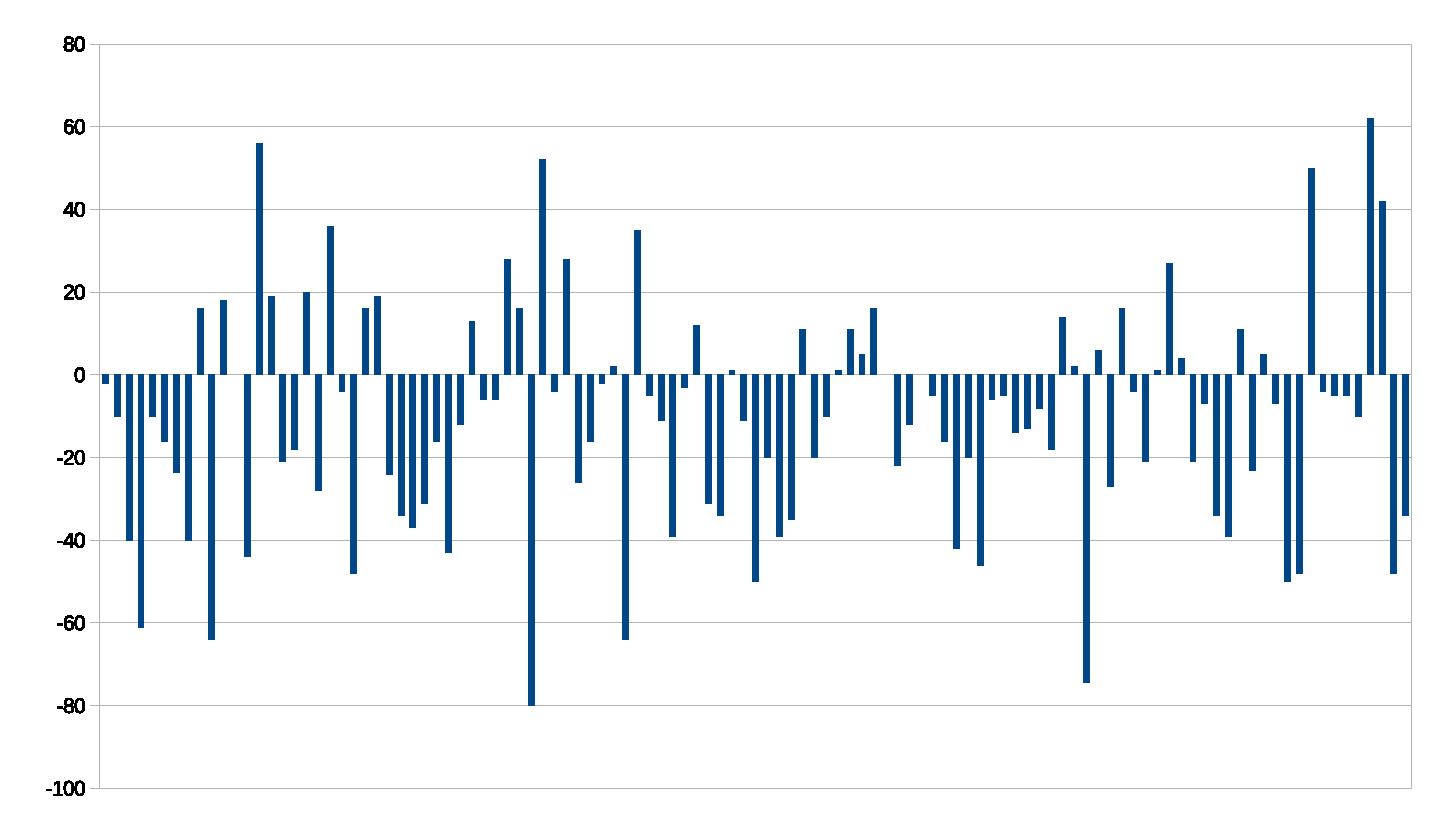
\includegraphics[width=10cm]{saldo_actual}
	\caption{Saldos \texttt{TOTAL} actual del professorat any 2018}
\end{figure}
\end{frame}


%Diapositiva 6 (2.)
\begin{frame}{Resultats \textit{Model Actual}, gràfics}
\begin{figure}
	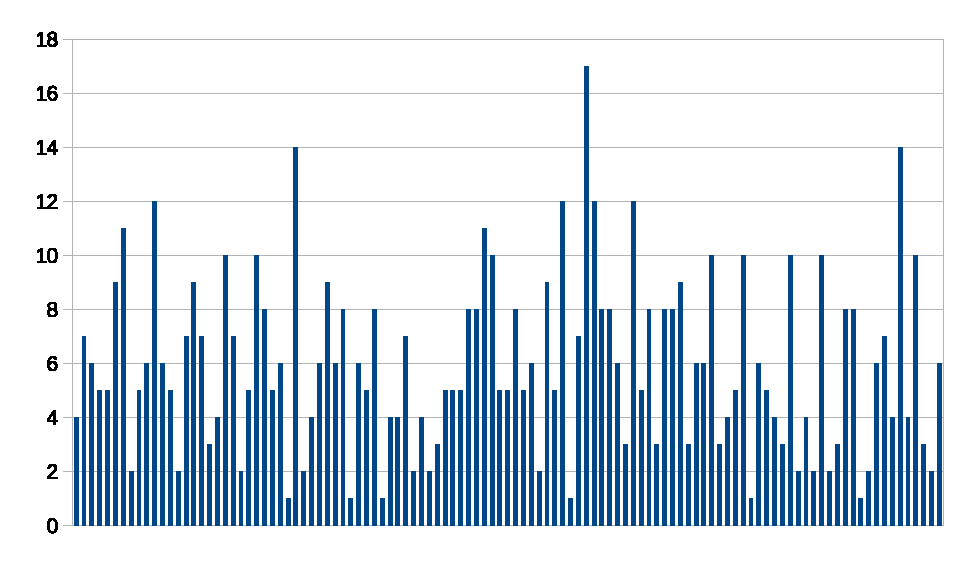
\includegraphics[width=10cm]{dispersio_actual}
	\caption{Dispersió \texttt{TOTAL} actual del professorat any 2018}
\end{figure}
\end{frame}


%Diapositiva 7 (2.)
\begin{frame}{$\mathbf 2.$ Anàlisis del \textit{Model Actual}}
\begin{columns}[t]
	%c1
	\begin{column}{.5\textwidth}
		\setbeamercolor{block title}{use=structure,fg=white,bg=green!75!black}
		%>\
		\begin{block}{Estat del model}
		
		\end{block}
	\end{column}
	%c2
	\begin{column}{.5\textwidth}
		\setbeamercolor{block title}{use=structure,fg=white,bg=green!75!black}
		\begin{block}{Valors rellevants}
			Lorem ipsum dolor sit amet,
			adipiscing elit. Upurus elit, vestibu
			consectetuer 
		\end{block}
		
\includegraphics[width=3.5cm]{eps}
	\end{column}
\end{columns}
\end{frame}

%Diapositiva 10 (3.)
\begin{frame}{$\mathbf 3.$ Model d’Optimització o d’investigació de sistemes}
\begin{columns}[t]
%c1
\begin{column}{.5\textwidth}
	\setbeamercolor{block title}{use=structure,fg=white,bg=orange!75!black}
	%>\
	\begin{block}{Una noció del model}
		[...la gracià està en escollir uns \emph{criteris raonables}
		a partir dels quals , i donades unes \textbf{restriccions}, definir una \textbf{funció objectiu} a optimitza...]
	\end{block}
\setbeamercolor{block title}{use=structure,fg=white,bg=orange!75!black}

\begin{block}{Optimització}
\texttt{\textbf{maximitzar} o \textbf{minimitzar}} \texttt{f}
\\ 
\texttt{Subjecte a}
\\
$\quad $ \texttt{\textbf{restriccions}}
\end{block}
\end{column}
%c2
\begin{column}{.5\textwidth}
	\setbeamercolor{block title}{use=structure,fg=white,bg=orange!75!black}
	\begin{block}{Un esquema}
		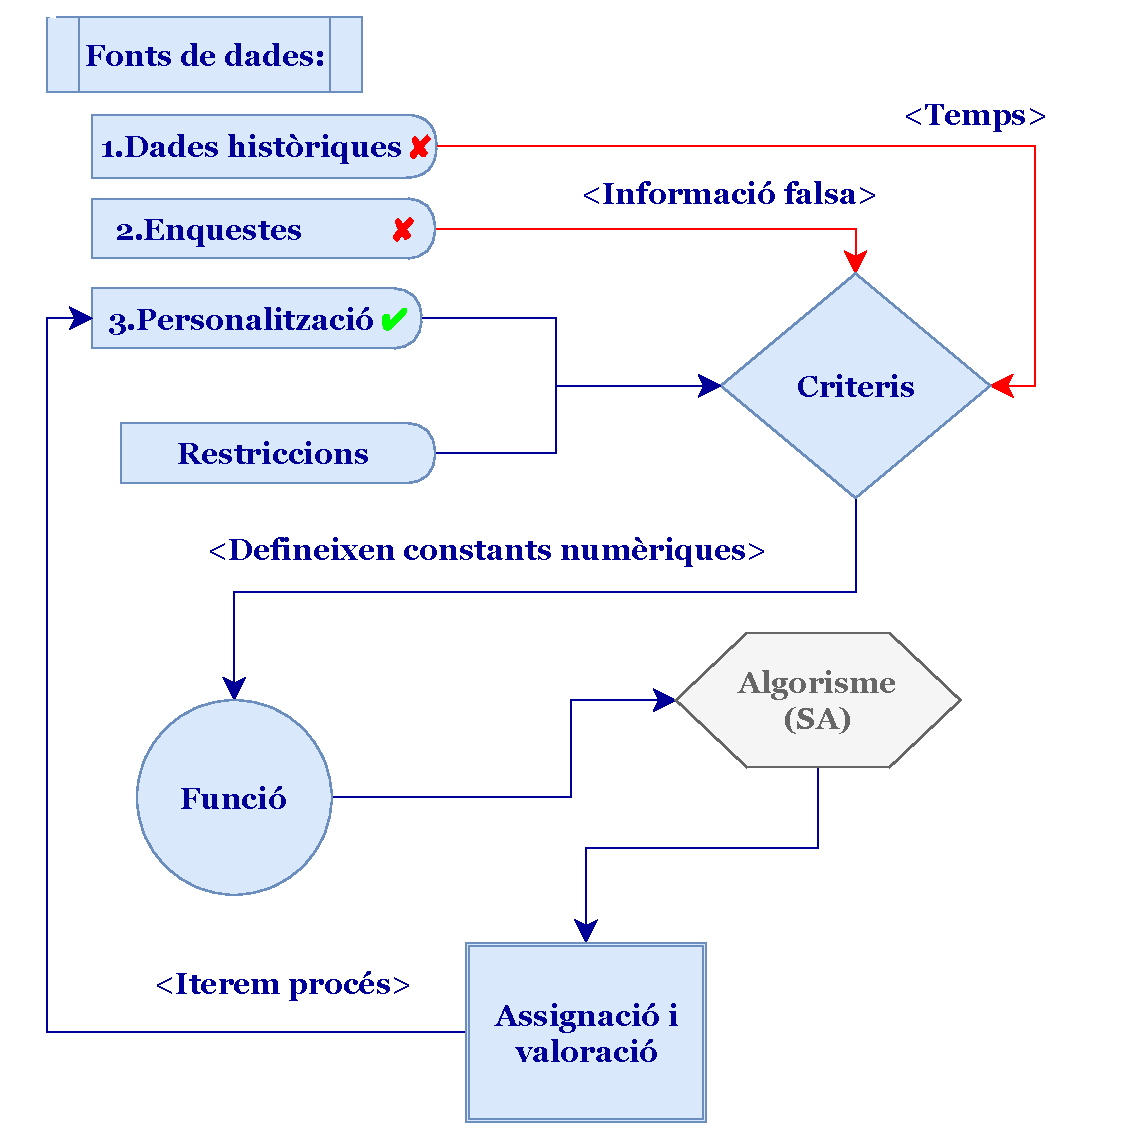
\includegraphics[width=5cm]{algor}
	\end{block}
\end{column}
\end{columns}
\end{frame}



%Diapositiva 10 (3.)
\begin{frame}{\textit{Biblioteca} de funcions i restriccions}
\begin{columns}[t]
	%c1
	\begin{column}{.5\textwidth}
		\setbeamercolor{block title}{use=structure,fg=white,bg=orange!75!black}
		%>\
		\begin{block}{Una noció del model}
			[...la gracià està en escollir uns \emph{criteris raonables}
			a partir dels quals , i donades unes \textbf{restriccions}, definir una \textbf{funció objectiu} a optimitza...]
		\end{block}
		\setbeamercolor{block title}{use=structure,fg=white,bg=orange!75!black}
		
		\begin{block}{Optimització}
			\texttt{\textbf{maximitzar} o \textbf{minimitzar}} \texttt{f}
			\\ 
			\texttt{Subjecte a}
			\\
			$\quad $ \texttt{\textbf{restriccions}}
		\end{block}
	\end{column}
	%c2
	\begin{column}{.5\textwidth}
		\setbeamercolor{block title}{use=structure,fg=white,bg=orange!75!black}
		\begin{block}{Un esquema}
			
\includegraphics[width=5cm]{eps}
		\end{block}
	\end{column}
\end{columns}
\end{frame}




\begin{frame}{\textit{Biblioteca} de funcions i restriccions}
\begin{figure}
	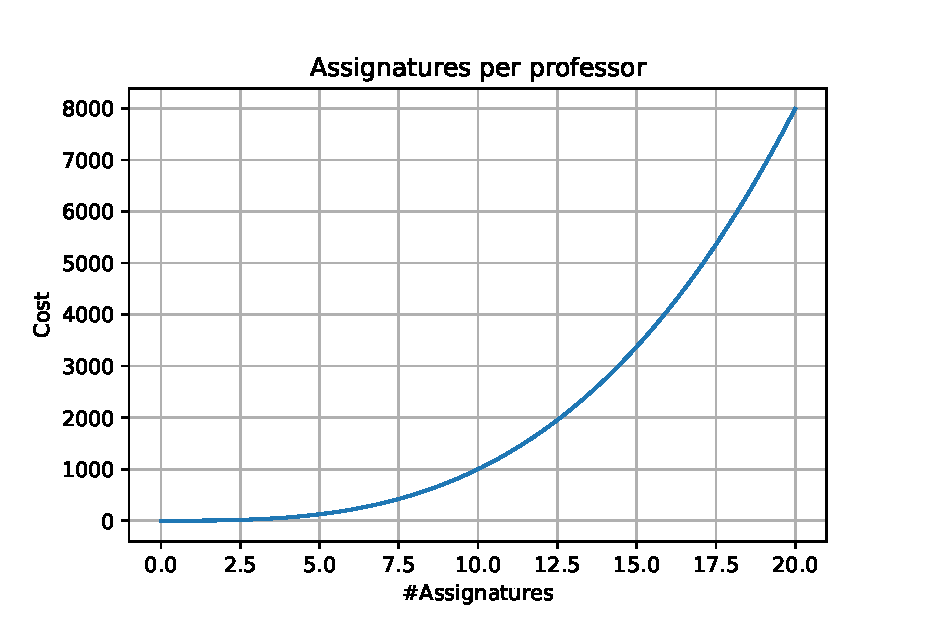
\includegraphics[width=9cm]{Assignatures}
	\caption{$x^3$}
\end{figure}
\end{frame}

\begin{frame}{\textit{Biblioteca} de funcions i restriccions}
\begin{figure}
	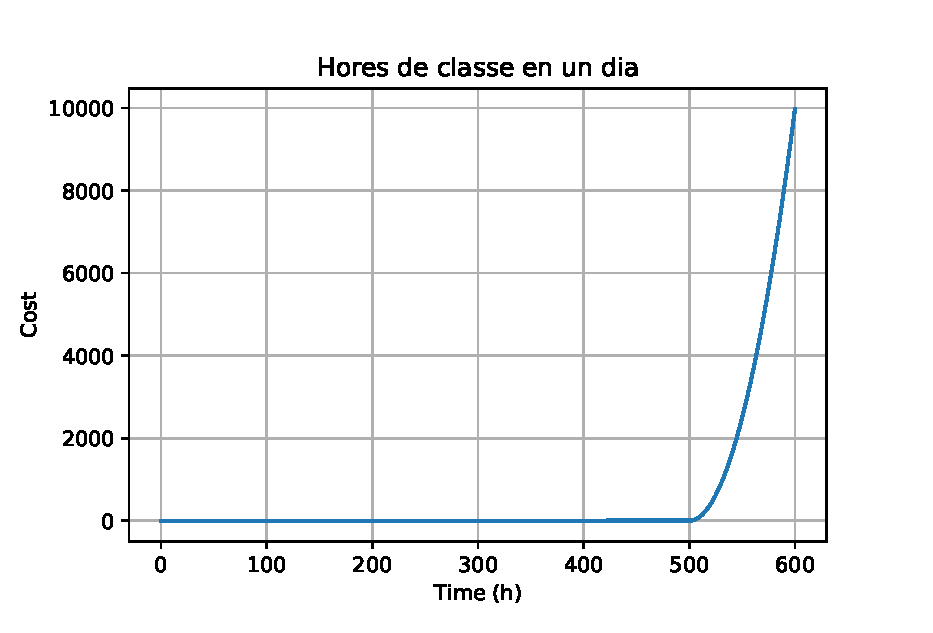
\includegraphics[width=9cm]{hores_dia}
	\caption{$(x-5000)^2$ si $x>5000$}
\end{figure}
\end{frame}

\begin{frame}{\textit{Biblioteca} de funcions i restriccions}
\begin{figure}
	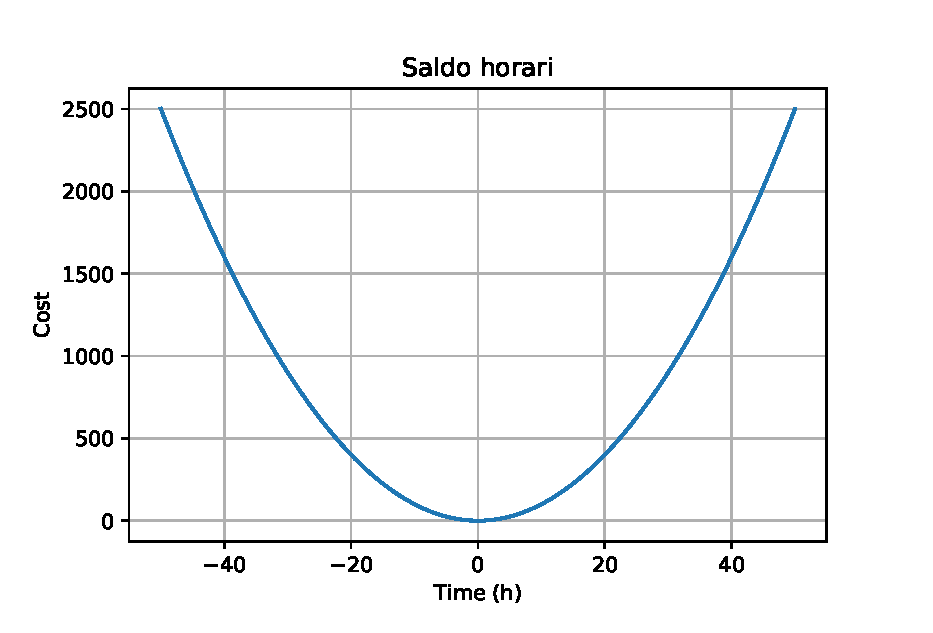
\includegraphics[width=9cm]{saldo}
	\caption{$x^2$}
\end{figure}
\end{frame}

\begin{frame}{\textit{Biblioteca} de funcions i restriccions}
\begin{figure}
	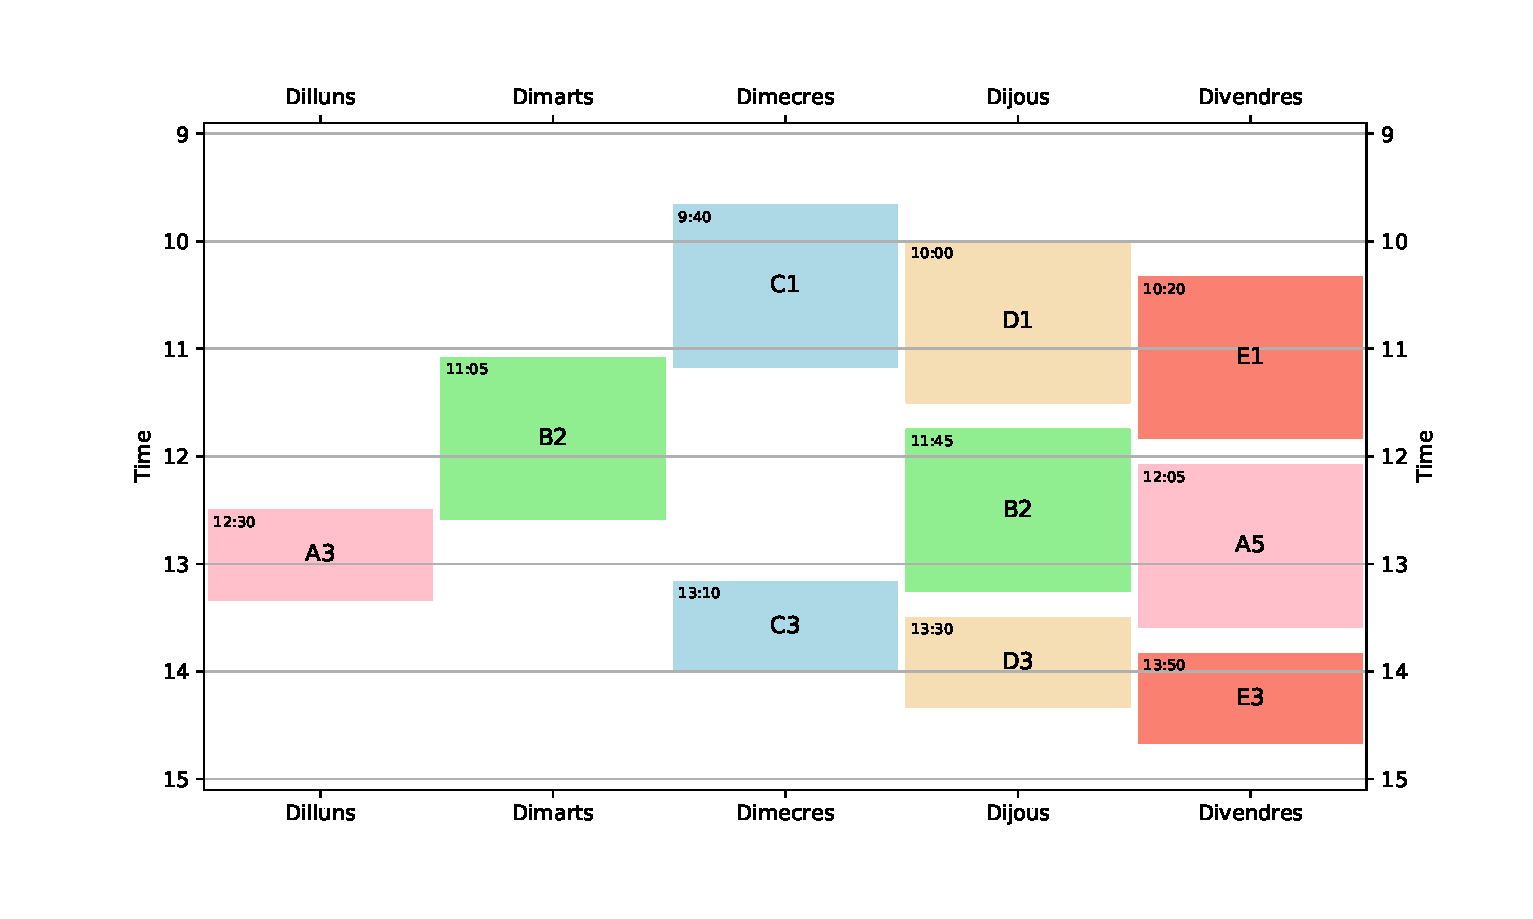
\includegraphics[width=9cm]{../plots/llibreria_funcs/horari}
	\caption{La distància entre classes es calcula entre dies}
\end{figure}
\end{frame}

\begin{frame}{\textit{Biblioteca} de funcions i restriccions}
\begin{figure}
	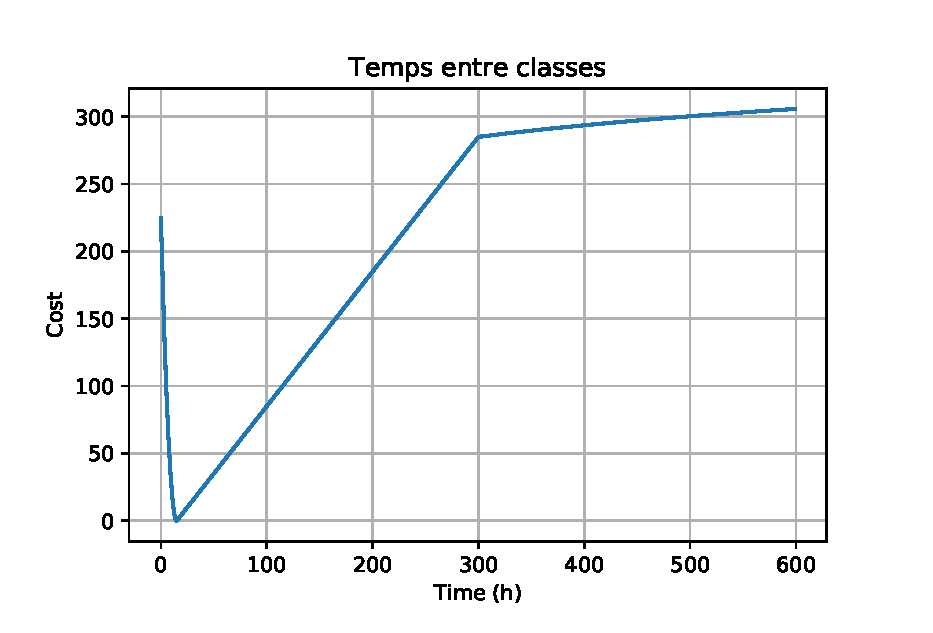
\includegraphics[width=9cm]{interclass}
	\caption{$x^2$, $x$ i $log(x)$}
\end{figure}
\end{frame}


%Diapositiva 10 (3.)
\begin{frame}{Resultats i limitacions del mode}
\begin{columns}[t]
	%c1
	\begin{column}{.5\textwidth}
		\setbeamercolor{block title}{use=structure,fg=white,bg=orange!75!black}
		%>\
		\begin{block}{Limitacions}
			Malgrat l'espai de solucions és finit, al ser de dimensió $|\mathbb{A}|\approx10^{5000}$, no podem garantir que la millor assignació que trobem és correspongui amb un  \textbf{mínim} de la \textbf{funció objectiu} ni donar cap altra garantia sobre la qualitat de la solució a la que arribaràn els algorismes d'optimització.
		\end{block}
		\setbeamercolor{block title}{use=structure,fg=white,bg=orange!75!black}
		
	\end{column}
	%c2
	\begin{column}{.5\textwidth}
		\setbeamercolor{block title}{use=structure,fg=white,bg=orange!75!black}
		
		\begin{block}{Justificació}
			\begin{itemize}
				\item \textbf{Solució factible}
				\item \textbf{Solució bona} ja que millora anys anterior.
			\end{itemize}
		\end{block}
		\begin{block}{Conclusions i resultats}
			A partir de simulacions concluïm que les solucions que trobem són bastant més bones que les obtingudes amb el model actual.
		\end{block}
	\end{column}
\end{columns}
\end{frame}


\begin{frame}{Conclusions funció}
\begin{figure}
	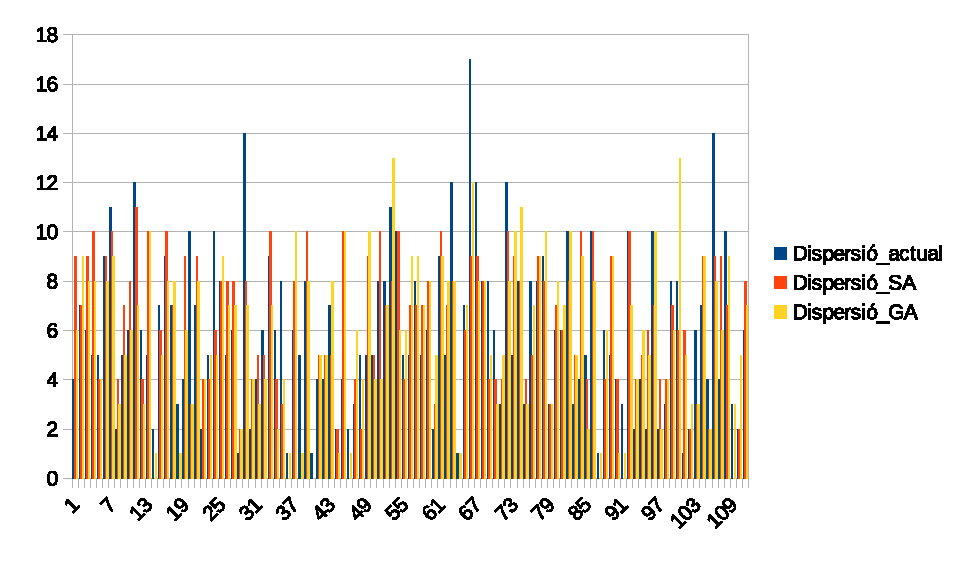
\includegraphics[width=9cm]{dispersio_diff_ga}
	\caption{Dispersió d'assignatures per professor}
\end{figure}
\end{frame}

\begin{frame}{Conclusions funció}
\begin{figure}
	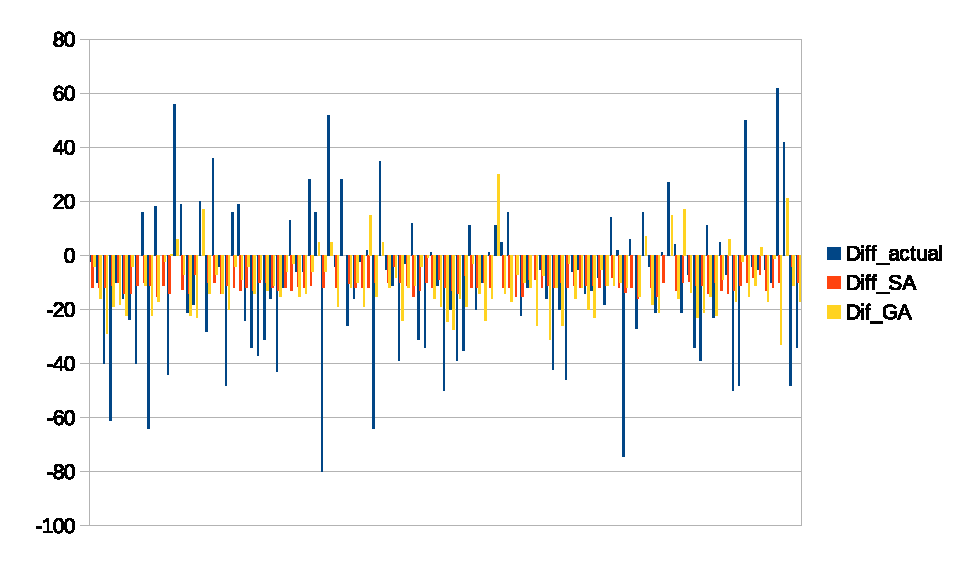
\includegraphics[width=9cm]{saldo_diff_ga}
	\begin{tabular}{c|c|c}
		\textbf{Model} & \textbf{Actual} & \textbf{Funció (SA)} \\
		Variància & 737.0676 & 14.7221 \\
		Suma absoluta & 2498 & 1156 \\
	\end{tabular}
\end{figure}
\end{frame}

%Diapositiva 11 (3.)
\begin{frame}{$\mathbf 4.$ \textit{Models} o \textit{Mètodes} per Subhastes}
\begin{columns}[t]
	%c1
	\begin{column}{.5\textwidth}
		\setbeamercolor{block title}{use=structure,fg=white,bg=cyan!75!black}
		%>\
		\begin{block}{Estat del model}
			Lorem ipsum dolor sit amet,
			consectetuer adipiscing elit. Upurus elit, vestibulum ut,
			placerat ac, adipiscing vitae,
			felis. Curabitur dictum gravida
			mauris. Nam arcu libero,
			nonummy eget, consectetuer ivulputate a, magna. Donec
			vehicula augue eu neque.
		\end{block}
	\end{column}
	%c2
	\begin{column}{.5\textwidth}
		\setbeamercolor{block title}{use=structure,fg=white,bg=cyan!75!black}
		\begin{block}{Valors rellevants}
			Lorem ipsum dolor sit amet,
			adipiscing elit. Upurus elit, vestibu
			consectetuer 
		\end{block}
		
\includegraphics[width=3.5cm]{eps}
	\end{column}
\end{columns}
\end{frame}
%Diapositiva 11 (3.)
\begin{frame}{$\mathbf 4.$ \textit{Models} o \textit{Mètodes} per Subhastes}
\begin{columns}[t]
	%c1
	\begin{column}{.5\textwidth}
		\setbeamercolor{block title}{use=structure,fg=white,bg=cyan!75!black}
		%>\
		\begin{block}{Estat del model}
			Lorem ipsum dolor sit amet,
			consectetuer adipiscing elit. Upurus elit, vestibulum ut,
			placerat ac, adipiscing vitae,
			felis. Curabitur dictum gravida
			mauris. Nam arcu libero,
			nonummy eget, consectetuer ivulputate a, magna. Donec
			vehicula augue eu neque.
		\end{block}
	\end{column}
	%c2
	\begin{column}{.5\textwidth}
		\setbeamercolor{block title}{use=structure,fg=white,bg=cyan!75!black}
		\begin{block}{Valors rellevants}
			Lorem ipsum dolor sit amet,
			adipiscing elit. Upurus elit, vestibu
			consectetuer 
		\end{block}
		
\includegraphics[width=3.5cm]{eps}
	\end{column}
\end{columns}
\end{frame}
%
%
%
%
%
%
%
%
%
%
%
%
\begin{frame}{Orientació i treball actual}
\begin{box1}{\normalsize Esquema treball (fins avui)}
\begin{itemize}
	\item Estudi del model actual.
	\\\textit{\color{redviolet} Entrevista A.Ruiz. i altres professors }
	\item Anàlisi de ineficiències.
	\\\textit{\color{redviolet} Discussió en sessions de classe.}
	\item Revalorització de les assignatures.
	\\\textit{\color{redviolet} Construcció de Models.}
	\item Ús d’eines com el llenguatge C o Python.
	\\\textit{\color{redviolet} Fer simulacions.}
\end{itemize}
\end{box1}

\end{frame}
\begin{frame}
\begin{box1}{ \normalsize Nous Models }
	\begin{enumerate}
		\small
		\item Model amb sistema de punts i subhastes. \textit{(Kiwis)}
		\item Model basat en algorisme.
		\item Model basat en algoritme i subhastes de Vickrey.
	\end{enumerate}
\end{box1}
{\Huge \centering
	$
	\quad \quad  \quad \quad  \quad \quad \Uparrow
	$
}
\begin{box1}{\normalsize Alguns criteris en la creació dels models }
	\small
	\begin{itemize}
		\item Volum de feina similar entre professors.
		\item Evitar estratègies guanyadores.
		\item Minimitzar dispersió.
		\item Satisfacció global en el repartiment.
		\item $\cdots$
	\end{itemize}
\end{box1}
\end{frame}
\begin{frame}{Model Actual} %Diapositiva 5 
\begin{box1}{\normalsize Alguns detalls sobre el model actual}
	\begin{itemize}
		\item 3 graus propis + 26 graus externs. \\ \textit{\footnotesize \color{blue} 500 sol·licituds $\approx$ 150 assignatures}
		\item 5 subdepartaments del departament. \\ \textit{ \footnotesize \color{blue} Assignatures 3r i 4rt graus propis.}
		\item  Ja ve fixat el horari, nombre de alumnes i la tipologia. \\ \textit{\footnotesize \color{blue} Això és si és una classe de problemes o de seminaris o $\cdots$}
		\item Les assignatures \textbf{només} són comptades per hores de classe realitzades.
	\end{itemize}
\end{box1}
\end{frame}

\begin{frame}{Model Actual} %Diapositiva 5 (Conceptes 1)
\begin{box1}{\normalsize Més detalls sobre el model actual}
	\begin{itemize}
		\item El nombre de hores que fa cada professor pot ser molt diferent. \\ \textit{\footnotesize \color{blue} oscil·la entre 60 i 240 hores per any}
		\item Actualment el model intenta minimitzar:
		\textit{\footnotesize \color{blue}
			\\-Dispersió: (\# assignatures)/professors
			\\-Deute personal}
	\end{itemize}
\end{box1}
El model complex i \textit{artesanal} \\\textbf{ $\Rightarrow$ Molta dedicació i conflictes en la presa de decisions.}
\\\textbf{ $\Rightarrow$ Sembla viable donar una proposta més curosa .}
\end{frame}
\begin{frame}{Model basat en punts \textit{Kiwis}}
\begin{tabular}{ m{10em}  m{2em}  m{10em} }
	\textbf{1. Enquesta}&{\Large +}&\textbf{2. Subhasta}\\
	\color{redviolet} $*$ Objectiu revaloritzar les assignatures. 
	&& \color{redviolet} $*$ Suposem que hi ha 6 matèries d'igual valor en hores: 1, 2 ,3 ,4 ,5 ,6.\\
	\color{redviolet} $*$ Per a evitar estratègies: descartar respostes $h’$ tal que $$|h-h’|>\frac{h}{2}$$&&
\includegraphics[width=5cm]{eps}
\end{tabular}
\end{frame}
\begin{frame}{Model basat en punts \textit{Kiwis}}
\begin{itemize}
	\item \textbf{A:} es queda amb les assignatures per les que més kiwis ha pagat fins a cobrir les hores. Les altres les perd i se li retornen els kiwis pagats.
	\item \textbf{B:} es queda igual.
	\item \textbf{C:} se li assignen les assignatures sobrants fins a cobrir les hores. 
\end{itemize}
\centering

\includegraphics[width=5cm]{eps}
\end{frame}
\begin{frame}{Problemàtica Subhastes}

\includegraphics[width=10cm]{eps}
\end{frame}
\begin{frame}{Model basat en \textit{Simulated annealing}}
\begin{box1}{\normalsize Alguns detalls sobre el model basat en SA}
	\begin{itemize}
		\item Idea central minimitzar una funció amb (SA).
		\item Funció additiva en la qual cada terme o sumand \textit{fa de representant} d'un criteri. 
		\item Funció $f$ avalua algunes de les $ \approx 10^{5000}$ possibilitats de repartiment i dóna un $a \in \R$ els que tinguin un valor més petit serà els candidats.
		\item Possibilitat de personalitzar criteris o definir funcions de preferència.
		\item Possibilitat de millores substancials dels resultats amb iteració del procés.
	\end{itemize}
\end{box1}
\end{frame}
\begin{frame}
\begin{box1}{\normalsize Un exemple de criteris concret}
	\begin{itemize}
		\item Terme que considera la equitat d'hores que ha de fer cada professor i reals  
		 $$f(x)=\sum_{i=1}^{112}(p_i-p'_i)^2+ \cdots + \cdots =a \in \R \quad \text{ amb } x \in \R^m$$
		 * on $p_i$ és el nombre de hores que ha de donar classe la persona docent i-èssima.
		 \\
		 * $p'_i$ és el nombre d'hores que donaria classes en una determinada assignació.
		 \\
		 * El que fa aquest terme en $f$ és penalitzar les diferencies entre $p_i$ i $p'_i$.
		 \\
		 * $\alpha=2,4,\cdots \Rightarrow$ S'han de triar les constants numèriques de la funció.
	\end{itemize}
\end{box1}
\end{frame}
\begin{frame}{Diagrama del model basat en \textit{Simulated} annealing}
\centering

\includegraphics[width=7cm]{eps}
\end{frame}
\begin{frame}{Primers Resultats, problema 1}
\centering

\includegraphics[width=10cm]{eps}
\end{frame}
\begin{frame}{Primers Resultats, resultat 1}
\centering

\includegraphics[width=10cm]{eps}
\end{frame}

\begin{frame}
\textit{\color{redviolet} \Huge Gràcies per la vostra atenció}
\end{frame}

\end{document}























%Diapositiva 2 (Expliquem el contigut breument del treball)
\begin{frame}{Esquema}
\begin{block}{Esquema presentació}
	\begin{enumerate}
		\item \textbf{Quan:} La presentació és o bé el 25 (de 9 a 12) o  bé el 28 (de 11 a 14) de març, no avançaran hora per  incentivar participació.
		\item \textbf{Temps:} uns 12 o 15 minuts, $[5,6]$ min per persona $ + \esp \{temps \esp de \esp preguntes\}$
		\item \textbf{Com:} La presentació ha d'estar dividida en 4 parts, ja que és sortejaran les parts entre els membres del grup. 
	\end{enumerate}
\end{block}
\end{frame} 
%Diapositiva 4
\begin{frame}{Una proposta de presentació}
\begin{block}{Una proposta de presentació:}
\begin{itemize}
	\item \textbf{Introducció i esquema treball:} Explicar en que consisteix el treball (fer un breu resum al nostre tema).
	\item \textbf{Primers conflictes:} Explicar primer Model per punts \textit{Kiwis} i problemàtica de la subhasta.
	\item \textbf{Algoritme i entrevista:}
	Comentar particularitats de l'algorisme i justificar amb entrevista.
	\item \textbf{Codi en C i primers resultats:}
	Donar imatges significatives dels primers resultats amb algorisme i explicar com el programa inicial en C ens va fer tenir una primera idea de possibles conflictes (comentar simultaneïtat). 
\end{itemize}
\end{block}
\end{frame}
\begin{frame}{21 i 25 de març} %Diapositiva 5 (Conceptes 1)
\begin{exampleblock}{Coses pendents}
\begin{itemize}
\item [21:] De cara a dijous s'han de pensar una llista de Criteris per a l'hora de programar el algoritme, quines \textit{coses} tingui en compte aquest. Dijous ja tindrem un resum de tot el fet fins ara.
\item [25:]De cara a dilluns s'hauria de tenir les diapositives, potser un parell per part (de les 4). I un breu resum d'una pàgina màxim i mitja mínim, per tal de poder tenir ideàs comuns. Ho podem parlar Dijous (Hi ha documents que és poden aprofitar penjats al Mahara).
\end{itemize}
\end{exampleblock}
\end{frame}
\begin{frame}
Totes les dades d'aquest document tenen caràcter de proposta, penso que el millor és discutir-ho dijous. Vaja que és per tenir una idea aproximada.
\end{frame}
****************************
****************************
**************************** 
****************************
****************************
****************************
****************************
**************************** 
****************************
****************************
%Aqui comença la presentació
